
% Default to the notebook output style

    


% Inherit from the specified cell style.




    
\documentclass[11pt]{article}

    
    
    \usepackage[T1]{fontenc}
    % Nicer default font (+ math font) than Computer Modern for most use cases
    \usepackage{mathpazo}

    % Basic figure setup, for now with no caption control since it's done
    % automatically by Pandoc (which extracts ![](path) syntax from Markdown).
    \usepackage{graphicx}
    % We will generate all images so they have a width \maxwidth. This means
    % that they will get their normal width if they fit onto the page, but
    % are scaled down if they would overflow the margins.
    \makeatletter
    \def\maxwidth{\ifdim\Gin@nat@width>\linewidth\linewidth
    \else\Gin@nat@width\fi}
    \makeatother
    \let\Oldincludegraphics\includegraphics
    % Set max figure width to be 80% of text width, for now hardcoded.
    \renewcommand{\includegraphics}[1]{\Oldincludegraphics[width=.8\maxwidth]{#1}}
    % Ensure that by default, figures have no caption (until we provide a
    % proper Figure object with a Caption API and a way to capture that
    % in the conversion process - todo).
    \usepackage{caption}
    \DeclareCaptionLabelFormat{nolabel}{}
    \captionsetup{labelformat=nolabel}

    \usepackage{adjustbox} % Used to constrain images to a maximum size 
    \usepackage{xcolor} % Allow colors to be defined
    \usepackage{enumerate} % Needed for markdown enumerations to work
    \usepackage{geometry} % Used to adjust the document margins
    \usepackage{amsmath} % Equations
    \usepackage{amssymb} % Equations
    \usepackage{textcomp} % defines textquotesingle
    % Hack from http://tex.stackexchange.com/a/47451/13684:
    \AtBeginDocument{%
        \def\PYZsq{\textquotesingle}% Upright quotes in Pygmentized code
    }
    \usepackage{upquote} % Upright quotes for verbatim code
    \usepackage{eurosym} % defines \euro
    \usepackage[mathletters]{ucs} % Extended unicode (utf-8) support
    \usepackage[utf8x]{inputenc} % Allow utf-8 characters in the tex document
    \usepackage{fancyvrb} % verbatim replacement that allows latex
    \usepackage{grffile} % extends the file name processing of package graphics 
                         % to support a larger range 
    % The hyperref package gives us a pdf with properly built
    % internal navigation ('pdf bookmarks' for the table of contents,
    % internal cross-reference links, web links for URLs, etc.)
    \usepackage{hyperref}
    \usepackage{longtable} % longtable support required by pandoc >1.10
    \usepackage{booktabs}  % table support for pandoc > 1.12.2
    \usepackage[inline]{enumitem} % IRkernel/repr support (it uses the enumerate* environment)
    \usepackage[normalem]{ulem} % ulem is needed to support strikethroughs (\sout)
                                % normalem makes italics be italics, not underlines
    

    
    
    % Colors for the hyperref package
    \definecolor{urlcolor}{rgb}{0,.145,.698}
    \definecolor{linkcolor}{rgb}{.71,0.21,0.01}
    \definecolor{citecolor}{rgb}{.12,.54,.11}

    % ANSI colors
    \definecolor{ansi-black}{HTML}{3E424D}
    \definecolor{ansi-black-intense}{HTML}{282C36}
    \definecolor{ansi-red}{HTML}{E75C58}
    \definecolor{ansi-red-intense}{HTML}{B22B31}
    \definecolor{ansi-green}{HTML}{00A250}
    \definecolor{ansi-green-intense}{HTML}{007427}
    \definecolor{ansi-yellow}{HTML}{DDB62B}
    \definecolor{ansi-yellow-intense}{HTML}{B27D12}
    \definecolor{ansi-blue}{HTML}{208FFB}
    \definecolor{ansi-blue-intense}{HTML}{0065CA}
    \definecolor{ansi-magenta}{HTML}{D160C4}
    \definecolor{ansi-magenta-intense}{HTML}{A03196}
    \definecolor{ansi-cyan}{HTML}{60C6C8}
    \definecolor{ansi-cyan-intense}{HTML}{258F8F}
    \definecolor{ansi-white}{HTML}{C5C1B4}
    \definecolor{ansi-white-intense}{HTML}{A1A6B2}

    % commands and environments needed by pandoc snippets
    % extracted from the output of `pandoc -s`
    \providecommand{\tightlist}{%
      \setlength{\itemsep}{0pt}\setlength{\parskip}{0pt}}
    \DefineVerbatimEnvironment{Highlighting}{Verbatim}{commandchars=\\\{\}}
    % Add ',fontsize=\small' for more characters per line
    \newenvironment{Shaded}{}{}
    \newcommand{\KeywordTok}[1]{\textcolor[rgb]{0.00,0.44,0.13}{\textbf{{#1}}}}
    \newcommand{\DataTypeTok}[1]{\textcolor[rgb]{0.56,0.13,0.00}{{#1}}}
    \newcommand{\DecValTok}[1]{\textcolor[rgb]{0.25,0.63,0.44}{{#1}}}
    \newcommand{\BaseNTok}[1]{\textcolor[rgb]{0.25,0.63,0.44}{{#1}}}
    \newcommand{\FloatTok}[1]{\textcolor[rgb]{0.25,0.63,0.44}{{#1}}}
    \newcommand{\CharTok}[1]{\textcolor[rgb]{0.25,0.44,0.63}{{#1}}}
    \newcommand{\StringTok}[1]{\textcolor[rgb]{0.25,0.44,0.63}{{#1}}}
    \newcommand{\CommentTok}[1]{\textcolor[rgb]{0.38,0.63,0.69}{\textit{{#1}}}}
    \newcommand{\OtherTok}[1]{\textcolor[rgb]{0.00,0.44,0.13}{{#1}}}
    \newcommand{\AlertTok}[1]{\textcolor[rgb]{1.00,0.00,0.00}{\textbf{{#1}}}}
    \newcommand{\FunctionTok}[1]{\textcolor[rgb]{0.02,0.16,0.49}{{#1}}}
    \newcommand{\RegionMarkerTok}[1]{{#1}}
    \newcommand{\ErrorTok}[1]{\textcolor[rgb]{1.00,0.00,0.00}{\textbf{{#1}}}}
    \newcommand{\NormalTok}[1]{{#1}}
    
    % Additional commands for more recent versions of Pandoc
    \newcommand{\ConstantTok}[1]{\textcolor[rgb]{0.53,0.00,0.00}{{#1}}}
    \newcommand{\SpecialCharTok}[1]{\textcolor[rgb]{0.25,0.44,0.63}{{#1}}}
    \newcommand{\VerbatimStringTok}[1]{\textcolor[rgb]{0.25,0.44,0.63}{{#1}}}
    \newcommand{\SpecialStringTok}[1]{\textcolor[rgb]{0.73,0.40,0.53}{{#1}}}
    \newcommand{\ImportTok}[1]{{#1}}
    \newcommand{\DocumentationTok}[1]{\textcolor[rgb]{0.73,0.13,0.13}{\textit{{#1}}}}
    \newcommand{\AnnotationTok}[1]{\textcolor[rgb]{0.38,0.63,0.69}{\textbf{\textit{{#1}}}}}
    \newcommand{\CommentVarTok}[1]{\textcolor[rgb]{0.38,0.63,0.69}{\textbf{\textit{{#1}}}}}
    \newcommand{\VariableTok}[1]{\textcolor[rgb]{0.10,0.09,0.49}{{#1}}}
    \newcommand{\ControlFlowTok}[1]{\textcolor[rgb]{0.00,0.44,0.13}{\textbf{{#1}}}}
    \newcommand{\OperatorTok}[1]{\textcolor[rgb]{0.40,0.40,0.40}{{#1}}}
    \newcommand{\BuiltInTok}[1]{{#1}}
    \newcommand{\ExtensionTok}[1]{{#1}}
    \newcommand{\PreprocessorTok}[1]{\textcolor[rgb]{0.74,0.48,0.00}{{#1}}}
    \newcommand{\AttributeTok}[1]{\textcolor[rgb]{0.49,0.56,0.16}{{#1}}}
    \newcommand{\InformationTok}[1]{\textcolor[rgb]{0.38,0.63,0.69}{\textbf{\textit{{#1}}}}}
    \newcommand{\WarningTok}[1]{\textcolor[rgb]{0.38,0.63,0.69}{\textbf{\textit{{#1}}}}}
    
    
    % Define a nice break command that doesn't care if a line doesn't already
    % exist.
    \def\br{\hspace*{\fill} \\* }
    % Math Jax compatability definitions
    \def\gt{>}
    \def\lt{<}
    % Document parameters
    \title{phase}
    
    
    

    % Pygments definitions
    
\makeatletter
\def\PY@reset{\let\PY@it=\relax \let\PY@bf=\relax%
    \let\PY@ul=\relax \let\PY@tc=\relax%
    \let\PY@bc=\relax \let\PY@ff=\relax}
\def\PY@tok#1{\csname PY@tok@#1\endcsname}
\def\PY@toks#1+{\ifx\relax#1\empty\else%
    \PY@tok{#1}\expandafter\PY@toks\fi}
\def\PY@do#1{\PY@bc{\PY@tc{\PY@ul{%
    \PY@it{\PY@bf{\PY@ff{#1}}}}}}}
\def\PY#1#2{\PY@reset\PY@toks#1+\relax+\PY@do{#2}}

\expandafter\def\csname PY@tok@w\endcsname{\def\PY@tc##1{\textcolor[rgb]{0.73,0.73,0.73}{##1}}}
\expandafter\def\csname PY@tok@c\endcsname{\let\PY@it=\textit\def\PY@tc##1{\textcolor[rgb]{0.25,0.50,0.50}{##1}}}
\expandafter\def\csname PY@tok@cp\endcsname{\def\PY@tc##1{\textcolor[rgb]{0.74,0.48,0.00}{##1}}}
\expandafter\def\csname PY@tok@k\endcsname{\let\PY@bf=\textbf\def\PY@tc##1{\textcolor[rgb]{0.00,0.50,0.00}{##1}}}
\expandafter\def\csname PY@tok@kp\endcsname{\def\PY@tc##1{\textcolor[rgb]{0.00,0.50,0.00}{##1}}}
\expandafter\def\csname PY@tok@kt\endcsname{\def\PY@tc##1{\textcolor[rgb]{0.69,0.00,0.25}{##1}}}
\expandafter\def\csname PY@tok@o\endcsname{\def\PY@tc##1{\textcolor[rgb]{0.40,0.40,0.40}{##1}}}
\expandafter\def\csname PY@tok@ow\endcsname{\let\PY@bf=\textbf\def\PY@tc##1{\textcolor[rgb]{0.67,0.13,1.00}{##1}}}
\expandafter\def\csname PY@tok@nb\endcsname{\def\PY@tc##1{\textcolor[rgb]{0.00,0.50,0.00}{##1}}}
\expandafter\def\csname PY@tok@nf\endcsname{\def\PY@tc##1{\textcolor[rgb]{0.00,0.00,1.00}{##1}}}
\expandafter\def\csname PY@tok@nc\endcsname{\let\PY@bf=\textbf\def\PY@tc##1{\textcolor[rgb]{0.00,0.00,1.00}{##1}}}
\expandafter\def\csname PY@tok@nn\endcsname{\let\PY@bf=\textbf\def\PY@tc##1{\textcolor[rgb]{0.00,0.00,1.00}{##1}}}
\expandafter\def\csname PY@tok@ne\endcsname{\let\PY@bf=\textbf\def\PY@tc##1{\textcolor[rgb]{0.82,0.25,0.23}{##1}}}
\expandafter\def\csname PY@tok@nv\endcsname{\def\PY@tc##1{\textcolor[rgb]{0.10,0.09,0.49}{##1}}}
\expandafter\def\csname PY@tok@no\endcsname{\def\PY@tc##1{\textcolor[rgb]{0.53,0.00,0.00}{##1}}}
\expandafter\def\csname PY@tok@nl\endcsname{\def\PY@tc##1{\textcolor[rgb]{0.63,0.63,0.00}{##1}}}
\expandafter\def\csname PY@tok@ni\endcsname{\let\PY@bf=\textbf\def\PY@tc##1{\textcolor[rgb]{0.60,0.60,0.60}{##1}}}
\expandafter\def\csname PY@tok@na\endcsname{\def\PY@tc##1{\textcolor[rgb]{0.49,0.56,0.16}{##1}}}
\expandafter\def\csname PY@tok@nt\endcsname{\let\PY@bf=\textbf\def\PY@tc##1{\textcolor[rgb]{0.00,0.50,0.00}{##1}}}
\expandafter\def\csname PY@tok@nd\endcsname{\def\PY@tc##1{\textcolor[rgb]{0.67,0.13,1.00}{##1}}}
\expandafter\def\csname PY@tok@s\endcsname{\def\PY@tc##1{\textcolor[rgb]{0.73,0.13,0.13}{##1}}}
\expandafter\def\csname PY@tok@sd\endcsname{\let\PY@it=\textit\def\PY@tc##1{\textcolor[rgb]{0.73,0.13,0.13}{##1}}}
\expandafter\def\csname PY@tok@si\endcsname{\let\PY@bf=\textbf\def\PY@tc##1{\textcolor[rgb]{0.73,0.40,0.53}{##1}}}
\expandafter\def\csname PY@tok@se\endcsname{\let\PY@bf=\textbf\def\PY@tc##1{\textcolor[rgb]{0.73,0.40,0.13}{##1}}}
\expandafter\def\csname PY@tok@sr\endcsname{\def\PY@tc##1{\textcolor[rgb]{0.73,0.40,0.53}{##1}}}
\expandafter\def\csname PY@tok@ss\endcsname{\def\PY@tc##1{\textcolor[rgb]{0.10,0.09,0.49}{##1}}}
\expandafter\def\csname PY@tok@sx\endcsname{\def\PY@tc##1{\textcolor[rgb]{0.00,0.50,0.00}{##1}}}
\expandafter\def\csname PY@tok@m\endcsname{\def\PY@tc##1{\textcolor[rgb]{0.40,0.40,0.40}{##1}}}
\expandafter\def\csname PY@tok@gh\endcsname{\let\PY@bf=\textbf\def\PY@tc##1{\textcolor[rgb]{0.00,0.00,0.50}{##1}}}
\expandafter\def\csname PY@tok@gu\endcsname{\let\PY@bf=\textbf\def\PY@tc##1{\textcolor[rgb]{0.50,0.00,0.50}{##1}}}
\expandafter\def\csname PY@tok@gd\endcsname{\def\PY@tc##1{\textcolor[rgb]{0.63,0.00,0.00}{##1}}}
\expandafter\def\csname PY@tok@gi\endcsname{\def\PY@tc##1{\textcolor[rgb]{0.00,0.63,0.00}{##1}}}
\expandafter\def\csname PY@tok@gr\endcsname{\def\PY@tc##1{\textcolor[rgb]{1.00,0.00,0.00}{##1}}}
\expandafter\def\csname PY@tok@ge\endcsname{\let\PY@it=\textit}
\expandafter\def\csname PY@tok@gs\endcsname{\let\PY@bf=\textbf}
\expandafter\def\csname PY@tok@gp\endcsname{\let\PY@bf=\textbf\def\PY@tc##1{\textcolor[rgb]{0.00,0.00,0.50}{##1}}}
\expandafter\def\csname PY@tok@go\endcsname{\def\PY@tc##1{\textcolor[rgb]{0.53,0.53,0.53}{##1}}}
\expandafter\def\csname PY@tok@gt\endcsname{\def\PY@tc##1{\textcolor[rgb]{0.00,0.27,0.87}{##1}}}
\expandafter\def\csname PY@tok@err\endcsname{\def\PY@bc##1{\setlength{\fboxsep}{0pt}\fcolorbox[rgb]{1.00,0.00,0.00}{1,1,1}{\strut ##1}}}
\expandafter\def\csname PY@tok@kc\endcsname{\let\PY@bf=\textbf\def\PY@tc##1{\textcolor[rgb]{0.00,0.50,0.00}{##1}}}
\expandafter\def\csname PY@tok@kd\endcsname{\let\PY@bf=\textbf\def\PY@tc##1{\textcolor[rgb]{0.00,0.50,0.00}{##1}}}
\expandafter\def\csname PY@tok@kn\endcsname{\let\PY@bf=\textbf\def\PY@tc##1{\textcolor[rgb]{0.00,0.50,0.00}{##1}}}
\expandafter\def\csname PY@tok@kr\endcsname{\let\PY@bf=\textbf\def\PY@tc##1{\textcolor[rgb]{0.00,0.50,0.00}{##1}}}
\expandafter\def\csname PY@tok@bp\endcsname{\def\PY@tc##1{\textcolor[rgb]{0.00,0.50,0.00}{##1}}}
\expandafter\def\csname PY@tok@fm\endcsname{\def\PY@tc##1{\textcolor[rgb]{0.00,0.00,1.00}{##1}}}
\expandafter\def\csname PY@tok@vc\endcsname{\def\PY@tc##1{\textcolor[rgb]{0.10,0.09,0.49}{##1}}}
\expandafter\def\csname PY@tok@vg\endcsname{\def\PY@tc##1{\textcolor[rgb]{0.10,0.09,0.49}{##1}}}
\expandafter\def\csname PY@tok@vi\endcsname{\def\PY@tc##1{\textcolor[rgb]{0.10,0.09,0.49}{##1}}}
\expandafter\def\csname PY@tok@vm\endcsname{\def\PY@tc##1{\textcolor[rgb]{0.10,0.09,0.49}{##1}}}
\expandafter\def\csname PY@tok@sa\endcsname{\def\PY@tc##1{\textcolor[rgb]{0.73,0.13,0.13}{##1}}}
\expandafter\def\csname PY@tok@sb\endcsname{\def\PY@tc##1{\textcolor[rgb]{0.73,0.13,0.13}{##1}}}
\expandafter\def\csname PY@tok@sc\endcsname{\def\PY@tc##1{\textcolor[rgb]{0.73,0.13,0.13}{##1}}}
\expandafter\def\csname PY@tok@dl\endcsname{\def\PY@tc##1{\textcolor[rgb]{0.73,0.13,0.13}{##1}}}
\expandafter\def\csname PY@tok@s2\endcsname{\def\PY@tc##1{\textcolor[rgb]{0.73,0.13,0.13}{##1}}}
\expandafter\def\csname PY@tok@sh\endcsname{\def\PY@tc##1{\textcolor[rgb]{0.73,0.13,0.13}{##1}}}
\expandafter\def\csname PY@tok@s1\endcsname{\def\PY@tc##1{\textcolor[rgb]{0.73,0.13,0.13}{##1}}}
\expandafter\def\csname PY@tok@mb\endcsname{\def\PY@tc##1{\textcolor[rgb]{0.40,0.40,0.40}{##1}}}
\expandafter\def\csname PY@tok@mf\endcsname{\def\PY@tc##1{\textcolor[rgb]{0.40,0.40,0.40}{##1}}}
\expandafter\def\csname PY@tok@mh\endcsname{\def\PY@tc##1{\textcolor[rgb]{0.40,0.40,0.40}{##1}}}
\expandafter\def\csname PY@tok@mi\endcsname{\def\PY@tc##1{\textcolor[rgb]{0.40,0.40,0.40}{##1}}}
\expandafter\def\csname PY@tok@il\endcsname{\def\PY@tc##1{\textcolor[rgb]{0.40,0.40,0.40}{##1}}}
\expandafter\def\csname PY@tok@mo\endcsname{\def\PY@tc##1{\textcolor[rgb]{0.40,0.40,0.40}{##1}}}
\expandafter\def\csname PY@tok@ch\endcsname{\let\PY@it=\textit\def\PY@tc##1{\textcolor[rgb]{0.25,0.50,0.50}{##1}}}
\expandafter\def\csname PY@tok@cm\endcsname{\let\PY@it=\textit\def\PY@tc##1{\textcolor[rgb]{0.25,0.50,0.50}{##1}}}
\expandafter\def\csname PY@tok@cpf\endcsname{\let\PY@it=\textit\def\PY@tc##1{\textcolor[rgb]{0.25,0.50,0.50}{##1}}}
\expandafter\def\csname PY@tok@c1\endcsname{\let\PY@it=\textit\def\PY@tc##1{\textcolor[rgb]{0.25,0.50,0.50}{##1}}}
\expandafter\def\csname PY@tok@cs\endcsname{\let\PY@it=\textit\def\PY@tc##1{\textcolor[rgb]{0.25,0.50,0.50}{##1}}}

\def\PYZbs{\char`\\}
\def\PYZus{\char`\_}
\def\PYZob{\char`\{}
\def\PYZcb{\char`\}}
\def\PYZca{\char`\^}
\def\PYZam{\char`\&}
\def\PYZlt{\char`\<}
\def\PYZgt{\char`\>}
\def\PYZsh{\char`\#}
\def\PYZpc{\char`\%}
\def\PYZdl{\char`\$}
\def\PYZhy{\char`\-}
\def\PYZsq{\char`\'}
\def\PYZdq{\char`\"}
\def\PYZti{\char`\~}
% for compatibility with earlier versions
\def\PYZat{@}
\def\PYZlb{[}
\def\PYZrb{]}
\makeatother


    % Exact colors from NB
    \definecolor{incolor}{rgb}{0.0, 0.0, 0.5}
    \definecolor{outcolor}{rgb}{0.545, 0.0, 0.0}



    
    % Prevent overflowing lines due to hard-to-break entities
    \sloppy 
    % Setup hyperref package
    \hypersetup{
      breaklinks=true,  % so long urls are correctly broken across lines
      colorlinks=true,
      urlcolor=urlcolor,
      linkcolor=linkcolor,
      citecolor=citecolor,
      }
    % Slightly bigger margins than the latex defaults
    
    \geometry{verbose,tmargin=1in,bmargin=1in,lmargin=1in,rmargin=1in}
    
    

    \begin{document}
    
    
    \maketitle
    
    

    
    \section{Hearing the phase of a
sound}\label{hearing-the-phase-of-a-sound}

In this notebook we will investigate the effect of phase on the
perceptual quality of a sound. It is often said that the human ear is
lergely insensitive to phase and that's why most of the equalization in
commercial-grade audio equipment takes place in the magnitude domain
only.

But is it really so? Let's find out.

    \begin{Verbatim}[commandchars=\\\{\}]
{\color{incolor}In [{\color{incolor}18}]:} \PY{o}{\PYZpc{}}\PY{k}{matplotlib} inline
         \PY{k+kn}{import} \PY{n+nn}{matplotlib}
         \PY{k+kn}{import} \PY{n+nn}{matplotlib}\PY{n+nn}{.}\PY{n+nn}{pyplot} \PY{k}{as} \PY{n+nn}{plt}
         \PY{k+kn}{import} \PY{n+nn}{numpy} \PY{k}{as} \PY{n+nn}{np}
         \PY{k+kn}{import} \PY{n+nn}{IPython}
         \PY{k+kn}{from} \PY{n+nn}{scipy}\PY{n+nn}{.}\PY{n+nn}{io} \PY{k}{import} \PY{n}{wavfile}
\end{Verbatim}


    \begin{Verbatim}[commandchars=\\\{\}]
{\color{incolor}In [{\color{incolor}19}]:} \PY{n}{plt}\PY{o}{.}\PY{n}{rcParams}\PY{p}{[}\PY{l+s+s2}{\PYZdq{}}\PY{l+s+s2}{figure.figsize}\PY{l+s+s2}{\PYZdq{}}\PY{p}{]} \PY{o}{=} \PY{p}{(}\PY{l+m+mi}{14}\PY{p}{,}\PY{l+m+mi}{4}\PY{p}{)}
\end{Verbatim}


    We will be synthesizing audio clips so let's set the sampling rate for
the rest of the not:

    \begin{Verbatim}[commandchars=\\\{\}]
{\color{incolor}In [{\color{incolor}20}]:} \PY{n}{Fs} \PY{o}{=} \PY{l+m+mi}{16000} \PY{c+c1}{\PYZsh{} sampling freqency}
         \PY{n}{TWOPI} \PY{o}{=} \PY{l+m+mi}{2} \PY{o}{*} \PY{n}{np}\PY{o}{.}\PY{n}{pi}
\end{Verbatim}


    We will be synthesizing and playing audio clips so let's define a
convenience function to "beautify" the resulting sound: basically, we
want a gentle fade-in and fade-out to avoid abrupt "clicks" when the
waveform begins and ends.

Also, there is a "bug" in the current version of IPython whereby audio
data is forcibly normalized prior to playing (see
\href{https://github.com/ipython/ipython/issues/8608}{here} for details;
this may have been solved in the meantime). On the other hand, we want
to avoid normalization in order to keep control over the volume of the
sound. A way to do so is to make sure that all audio clips have at least
one sample at a pre-defined maximum value, and this value is the same
for all clips. To do so we add a slow "tail" to the data which will not
result in an audible sound but will set a common maximum value in all
clips.

    \begin{Verbatim}[commandchars=\\\{\}]
{\color{incolor}In [{\color{incolor}1}]:} \PY{k}{def} \PY{n+nf}{prepare}\PY{p}{(}\PY{n}{x}\PY{p}{,} \PY{n}{max\PYZus{}value} \PY{o}{=} \PY{l+m+mi}{3}\PY{p}{)}\PY{p}{:}
            \PY{n}{N} \PY{o}{=} \PY{n+nb}{len}\PY{p}{(}\PY{n}{x}\PY{p}{)}
            \PY{c+c1}{\PYZsh{} fade\PYZhy{}in and fade\PYZhy{}out times max 0.2 seconds}
            \PY{n}{tf} \PY{o}{=} \PY{n+nb}{min}\PY{p}{(}\PY{n+nb}{int}\PY{p}{(}\PY{l+m+mf}{0.2} \PY{o}{*} \PY{n}{Fs}\PY{p}{)}\PY{p}{,} \PY{n+nb}{int}\PY{p}{(}\PY{l+m+mf}{0.1} \PY{o}{*} \PY{n}{N}\PY{p}{)}\PY{p}{)}
            \PY{k}{for} \PY{n}{n} \PY{o+ow}{in} \PY{n+nb}{range}\PY{p}{(}\PY{l+m+mi}{0}\PY{p}{,} \PY{n+nb}{int}\PY{p}{(}\PY{n}{tf}\PY{p}{)}\PY{p}{)}\PY{p}{:}
                \PY{n}{s} \PY{o}{=} \PY{n+nb}{float}\PY{p}{(}\PY{n}{n}\PY{p}{)} \PY{o}{/} \PY{n+nb}{float}\PY{p}{(}\PY{n}{tf}\PY{p}{)}
                \PY{n}{x}\PY{p}{[}\PY{n}{n}\PY{p}{]} \PY{o}{*}\PY{o}{=} \PY{n}{s}
                \PY{n}{x}\PY{p}{[}\PY{n}{N}\PY{o}{\PYZhy{}}\PY{n}{n}\PY{o}{\PYZhy{}}\PY{l+m+mi}{1}\PY{p}{]} \PY{o}{*}\PY{o}{=} \PY{n}{s}
            \PY{c+c1}{\PYZsh{} let\PYZsq{}s append an anti\PYZhy{}normalization tail; drawback is one second of silence in the end}
            \PY{n}{x} \PY{o}{=} \PY{n}{np}\PY{o}{.}\PY{n}{concatenate}\PY{p}{(}\PY{p}{(}\PY{n}{x}\PY{p}{,} \PY{n}{np}\PY{o}{.}\PY{n}{linspace}\PY{p}{(}\PY{l+m+mi}{0}\PY{p}{,} \PY{n}{max\PYZus{}value}\PY{p}{,} \PY{n+nb}{int}\PY{p}{(}\PY{n}{Fs}\PY{o}{/}\PY{l+m+mi}{2}\PY{p}{)}\PY{p}{)}\PY{p}{,} \PY{n}{np}\PY{o}{.}\PY{n}{linspace}\PY{p}{(}\PY{n}{max\PYZus{}value}\PY{p}{,} \PY{l+m+mi}{0}\PY{p}{,} \PY{n+nb}{int}\PY{p}{(}\PY{n}{Fs}\PY{o}{/}\PY{l+m+mi}{2}\PY{p}{)}\PY{p}{)}\PY{p}{)}\PY{p}{)}
            \PY{k}{return} \PY{n}{x}
\end{Verbatim}


    \subsection{1) Sustained sounds}\label{sustained-sounds}

The first experiment will use sustained sounds, i.e. waveform whose
global envelope does not change in time. A periodic sustained waveform
is simply the sum of harmonically-related sinusoidal components, i.e. a
set of sines or cosines with different amplitudes and phases at
frequencies multiple of a fundamental. The fundamental frequency is also
known as the pitch of the sound.

A class of instruments that produce good sustained sounds is the
woodwinds (clarinet, saxophone, etc). The mechanics of sound generation
in woodwinds are beyond the scope of this notebook and plenty of
references can be found on the internet. For our purposes we will choose
to simulate a clarinet according to the analysis described
\href{http://www.phy.mtu.edu/~suits/clarinet.html}{here}.

\begin{figure}
\centering
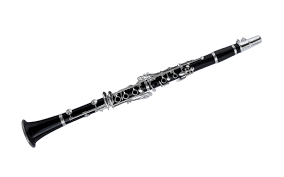
\includegraphics{clarinet.png}
\caption{title}
\end{figure}

A clarinet-like sustained sound will contain frequencies at odd
multiples of the fundamental. We will just keep the fundamental and five
harmonics and we be able to specify the initial phase offset for each
component:

    \begin{Verbatim}[commandchars=\\\{\}]
{\color{incolor}In [{\color{incolor}50}]:} \PY{k}{def} \PY{n+nf}{clarinet}\PY{p}{(}\PY{n}{f}\PY{p}{,} \PY{n}{phase} \PY{o}{=} \PY{p}{[}\PY{p}{]}\PY{p}{)}\PY{p}{:}
             \PY{c+c1}{\PYZsh{} length in seconds of audio clips}
             \PY{n}{T} \PY{o}{=} \PY{l+m+mi}{3}
             
             \PY{c+c1}{\PYZsh{} we will keep 5 harmonics and the fundamental}
             \PY{c+c1}{\PYZsh{} amplitude of components: }
             \PY{n}{ha} \PY{o}{=} \PY{p}{[}\PY{l+m+mf}{0.75}\PY{p}{,} \PY{l+m+mf}{0.5}\PY{p}{,} \PY{l+m+mf}{0.14}\PY{p}{,} \PY{l+m+mf}{0.5}\PY{p}{,} \PY{l+m+mf}{0.12}\PY{p}{,} \PY{l+m+mf}{0.17}\PY{p}{]}
             
             \PY{c+c1}{\PYZsh{} phase}
             \PY{n}{phase} \PY{o}{=} \PY{n}{np}\PY{o}{.}\PY{n}{concatenate}\PY{p}{(}\PY{p}{(}\PY{n}{phase}\PY{p}{,} \PY{n}{np}\PY{o}{.}\PY{n}{zeros}\PY{p}{(}\PY{n+nb}{len}\PY{p}{(}\PY{n}{ha}\PY{p}{)}\PY{o}{\PYZhy{}}\PY{n+nb}{len}\PY{p}{(}\PY{n}{phase}\PY{p}{)}\PY{p}{)}\PY{p}{)}\PY{p}{)}
         
             \PY{n}{x} \PY{o}{=} \PY{n}{np}\PY{o}{.}\PY{n}{zeros}\PY{p}{(}\PY{p}{(}\PY{n}{T} \PY{o}{*} \PY{n}{Fs}\PY{p}{)}\PY{p}{)}
             \PY{c+c1}{\PYZsh{} clarinet has only odd harmonics}
             \PY{n}{n} \PY{o}{=} \PY{n}{np}\PY{o}{.}\PY{n}{arange}\PY{p}{(}\PY{n+nb}{len}\PY{p}{(}\PY{n}{x}\PY{p}{)}\PY{p}{)}
             \PY{k}{for} \PY{n}{k}\PY{p}{,} \PY{n}{h} \PY{o+ow}{in} \PY{n+nb}{enumerate}\PY{p}{(}\PY{n}{ha}\PY{p}{)}\PY{p}{:}
                 \PY{n}{x} \PY{o}{+}\PY{o}{=} \PY{n}{h} \PY{o}{*} \PY{n}{np}\PY{o}{.}\PY{n}{sin}\PY{p}{(}\PY{n}{phase}\PY{p}{[}\PY{n}{k}\PY{p}{]} \PY{o}{+} \PY{n}{TWOPI} \PY{o}{*} \PY{p}{(}\PY{l+m+mi}{2}\PY{o}{*}\PY{n}{k} \PY{o}{+} \PY{l+m+mi}{1}\PY{p}{)} \PY{o}{*} \PY{p}{(}\PY{n+nb}{float}\PY{p}{(}\PY{n}{f}\PY{p}{)}\PY{o}{/}\PY{n}{Fs}\PY{p}{)} \PY{o}{*} \PY{n}{n}\PY{p}{)}
             \PY{k}{return} \PY{n}{x}
\end{Verbatim}


    \begin{Verbatim}[commandchars=\\\{\}]
{\color{incolor}In [{\color{incolor}51}]:} \PY{c+c1}{\PYZsh{} fundamental frequency: D4}
         \PY{n}{D4} \PY{o}{=} \PY{l+m+mf}{293.665}
         \PY{n}{x} \PY{o}{=} \PY{n}{clarinet}\PY{p}{(}\PY{n}{D4}\PY{p}{)}
         
         \PY{c+c1}{\PYZsh{} let\PYZsq{}s look at the waveform, nice odd\PYZhy{}harmonics shape:    }
         \PY{n}{plt}\PY{o}{.}\PY{n}{plot}\PY{p}{(}\PY{n}{x}\PY{p}{[}\PY{l+m+mi}{0}\PY{p}{:}\PY{l+m+mi}{300}\PY{p}{]}\PY{p}{)}
         \PY{n}{plt}\PY{o}{.}\PY{n}{show}\PY{p}{(}\PY{p}{)}
         
         \PY{c+c1}{\PYZsh{} and of course we can play it (using our preparing function):}
         \PY{n}{IPython}\PY{o}{.}\PY{n}{display}\PY{o}{.}\PY{n}{Audio}\PY{p}{(}\PY{n}{prepare}\PY{p}{(}\PY{n}{x}\PY{p}{)}\PY{p}{,} \PY{n}{rate}\PY{o}{=}\PY{n}{Fs}\PY{p}{)}
\end{Verbatim}


    \begin{center}
    \adjustimage{max size={0.9\linewidth}{0.9\paperheight}}{output_9_0.png}
    \end{center}
    { \hspace*{\fill} \\}
    
\begin{Verbatim}[commandchars=\\\{\}]
{\color{outcolor}Out[{\color{outcolor}51}]:} <IPython.lib.display.Audio object>
\end{Verbatim}
            
    Ok, so it's not the best clarinet sound in the universe but it's not bad
for just a few lines of code. Now let's see how changing the phase
affects the sound. Let's just use random phase offsets for the
components: we can see that the waveform doesn't look too nice anymore:

    \begin{Verbatim}[commandchars=\\\{\}]
{\color{incolor}In [{\color{incolor}52}]:} \PY{n}{xrp} \PY{o}{=} \PY{n}{clarinet}\PY{p}{(}\PY{n}{D4}\PY{p}{,} \PY{p}{[}\PY{l+m+mf}{3.84}\PY{p}{,} \PY{l+m+mf}{0.90}\PY{p}{,} \PY{l+m+mf}{3.98}\PY{p}{,} \PY{l+m+mf}{4.50}\PY{p}{,} \PY{l+m+mf}{4.80}\PY{p}{,} \PY{l+m+mf}{2.96}\PY{p}{]}\PY{p}{)}
         
         \PY{n}{plt}\PY{o}{.}\PY{n}{plot}\PY{p}{(}\PY{n}{xrp}\PY{p}{[}\PY{l+m+mi}{0}\PY{p}{:}\PY{l+m+mi}{300}\PY{p}{]}\PY{p}{)}
         \PY{n}{plt}\PY{o}{.}\PY{n}{show}\PY{p}{(}\PY{p}{)}
\end{Verbatim}


    \begin{center}
    \adjustimage{max size={0.9\linewidth}{0.9\paperheight}}{output_11_0.png}
    \end{center}
    { \hspace*{\fill} \\}
    
    \begin{Verbatim}[commandchars=\\\{\}]
{\color{incolor}In [{\color{incolor}53}]:} \PY{c+c1}{\PYZsh{} but if we play it, it sounds the same!    }
         \PY{n}{IPython}\PY{o}{.}\PY{n}{display}\PY{o}{.}\PY{n}{Audio}\PY{p}{(}\PY{n}{prepare}\PY{p}{(}\PY{n}{xrp}\PY{p}{)}\PY{p}{,} \PY{n}{rate}\PY{o}{=}\PY{n}{Fs}\PY{p}{)}
\end{Verbatim}


\begin{Verbatim}[commandchars=\\\{\}]
{\color{outcolor}Out[{\color{outcolor}53}]:} <IPython.lib.display.Audio object>
\end{Verbatim}
            
    OK, so it seems that phase is not important after all. To check once
again, run the following notebook cell as many times as you want and see
if you can tell the difference between the original zero-phase and a
random-phase sustained note (the phases will be different every time you
run the cell):

    \begin{Verbatim}[commandchars=\\\{\}]
{\color{incolor}In [{\color{incolor}54}]:} \PY{n}{xrp} \PY{o}{=} \PY{n}{clarinet}\PY{p}{(}\PY{n}{D4}\PY{p}{,} \PY{n}{np}\PY{o}{.}\PY{n}{random}\PY{o}{.}\PY{n}{rand}\PY{p}{(}\PY{l+m+mi}{6}\PY{p}{)} \PY{o}{*} \PY{n}{TWOPI}\PY{p}{)}
         \PY{n}{plt}\PY{o}{.}\PY{n}{plot}\PY{p}{(}\PY{n}{xrp}\PY{p}{[}\PY{l+m+mi}{0}\PY{p}{:}\PY{l+m+mi}{300}\PY{p}{]}\PY{p}{)}
         \PY{n}{plt}\PY{o}{.}\PY{n}{show}\PY{p}{(}\PY{p}{)}  
         \PY{n}{IPython}\PY{o}{.}\PY{n}{display}\PY{o}{.}\PY{n}{display}\PY{p}{(}\PY{n}{IPython}\PY{o}{.}\PY{n}{display}\PY{o}{.}\PY{n}{Audio}\PY{p}{(}\PY{n}{prepare}\PY{p}{(}\PY{n}{x}\PY{p}{)}\PY{p}{,} \PY{n}{rate}\PY{o}{=}\PY{n}{Fs}\PY{p}{)}\PY{p}{)}
         \PY{n}{IPython}\PY{o}{.}\PY{n}{display}\PY{o}{.}\PY{n}{display}\PY{p}{(}\PY{n}{IPython}\PY{o}{.}\PY{n}{display}\PY{o}{.}\PY{n}{Audio}\PY{p}{(}\PY{n}{prepare}\PY{p}{(}\PY{n}{xrp}\PY{p}{)}\PY{p}{,} \PY{n}{rate}\PY{o}{=}\PY{n}{Fs}\PY{p}{)}\PY{p}{)}
\end{Verbatim}


    \begin{center}
    \adjustimage{max size={0.9\linewidth}{0.9\paperheight}}{output_14_0.png}
    \end{center}
    { \hspace*{\fill} \\}
    
    
    \begin{verbatim}
<IPython.lib.display.Audio object>
    \end{verbatim}

    
    
    \begin{verbatim}
<IPython.lib.display.Audio object>
    \end{verbatim}

    
    \subsection{1) Dynamic sounds}\label{dynamic-sounds}

In the second experiment we will use real-world dynamic sounds, i.e.
sounds that display time-varying characteristics. Typically, a physical
musical instrument will produce sounds whose envelope displays four
subsequent portions:

\begin{itemize}
\tightlist
\item
  the \textbf{attack} time is the time taken for the sound to go from
  silence to max amplitude
\item
  the \textbf{decay} time is the time taken for the sound to decrease to
  sustain level
\item
  the \textbf{sustain} time is the time during the sound is kept at the
  same amplitude
\item
  the \textbf{release} time is the time taken for sound to go to zero
  after the stimulation is stopped.
\end{itemize}

\begin{figure}
\centering
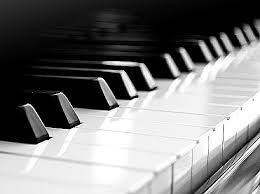
\includegraphics{piano.jpg}
\caption{title}
\end{figure}

Consider for instance a piano note: the attack time is very quick (the
hammer hits the string); the decay is quite rapid as the string settles
into harmonic equilibrium but there is no sustain since once the hammer
hits, the stimulation ends. So a piano note has a distinct volume
envelope that rises very fast and then releases slowly:

    \begin{Verbatim}[commandchars=\\\{\}]
{\color{incolor}In [{\color{incolor}55}]:} \PY{k+kn}{from} \PY{n+nn}{scipy}\PY{n+nn}{.}\PY{n+nn}{io} \PY{k}{import} \PY{n}{wavfile}
         \PY{n}{Fs}\PY{p}{,} \PY{n}{x} \PY{o}{=} \PY{n}{wavfile}\PY{o}{.}\PY{n}{read}\PY{p}{(}\PY{l+s+s2}{\PYZdq{}}\PY{l+s+s2}{piano.wav}\PY{l+s+s2}{\PYZdq{}}\PY{p}{)}
         \PY{n}{plt}\PY{o}{.}\PY{n}{plot}\PY{p}{(}\PY{n}{x}\PY{p}{)}
         \PY{n}{plt}\PY{o}{.}\PY{n}{show}\PY{p}{(}\PY{p}{)} 
         \PY{n}{IPython}\PY{o}{.}\PY{n}{display}\PY{o}{.}\PY{n}{Audio}\PY{p}{(}\PY{n}{x}\PY{p}{,} \PY{n}{rate}\PY{o}{=}\PY{n}{Fs}\PY{p}{)}
\end{Verbatim}


    \begin{center}
    \adjustimage{max size={0.9\linewidth}{0.9\paperheight}}{output_16_0.png}
    \end{center}
    { \hspace*{\fill} \\}
    
\begin{Verbatim}[commandchars=\\\{\}]
{\color{outcolor}Out[{\color{outcolor}55}]:} <IPython.lib.display.Audio object>
\end{Verbatim}
            
    By now we know that the "shape" of a waveform is largely encoded in the
phase. It is no surprise, therefore, that if we mess up with the phase
of the piano sample above, we will get something that looks very
different.

To see this, let's take the DFT of the audio data, set the phase to zero
and take the IDFT:

    \begin{Verbatim}[commandchars=\\\{\}]
{\color{incolor}In [{\color{incolor}56}]:} \PY{c+c1}{\PYZsh{} first some prep work; let\PYZsq{}s make sure that}
         \PY{c+c1}{\PYZsh{}  the length of the signal is even }
         \PY{c+c1}{\PYZsh{}  (it will be useful later)}
         \PY{k}{if} \PY{n+nb}{len}\PY{p}{(}\PY{n}{x}\PY{p}{)} \PY{o}{\PYZpc{}} \PY{l+m+mi}{2} \PY{o}{!=} \PY{l+m+mi}{0}\PY{p}{:}
             \PY{n}{x} \PY{o}{=} \PY{n}{x}\PY{p}{[}\PY{p}{:}\PY{o}{\PYZhy{}}\PY{l+m+mi}{1}\PY{p}{]}
         
         \PY{c+c1}{\PYZsh{} let\PYZsq{}s also store the maximum value for our }
         \PY{c+c1}{\PYZsh{}  \PYZdq{}prepare\PYZdq{} function   }
         \PY{n}{mv} \PY{o}{=} \PY{n+nb}{int}\PY{p}{(}\PY{n+nb}{max}\PY{p}{(}\PY{n+nb}{abs}\PY{p}{(}\PY{n}{x}\PY{p}{)}\PY{p}{)} \PY{o}{*} \PY{l+m+mf}{1.2}\PY{p}{)}
\end{Verbatim}


    \begin{Verbatim}[commandchars=\\\{\}]
{\color{incolor}In [{\color{incolor}57}]:} \PY{c+c1}{\PYZsh{} Let\PYZsq{}s take the Fourier transform}
         \PY{n}{X} \PY{o}{=} \PY{n}{np}\PY{o}{.}\PY{n}{fft}\PY{o}{.}\PY{n}{fft}\PY{p}{(}\PY{n}{x}\PY{p}{)}
         
         \PY{c+c1}{\PYZsh{} we can plot the DFT and verify we have a nice }
         \PY{c+c1}{\PYZsh{}  harmonic spectrum}
         \PY{n}{plt}\PY{o}{.}\PY{n}{plot}\PY{p}{(}\PY{n}{np}\PY{o}{.}\PY{n}{abs}\PY{p}{(}\PY{n}{X}\PY{p}{[}\PY{l+m+mi}{0}\PY{p}{:}\PY{n+nb}{int}\PY{p}{(}\PY{n+nb}{len}\PY{p}{(}\PY{n}{X}\PY{p}{)}\PY{o}{/}\PY{l+m+mi}{2}\PY{p}{)}\PY{p}{]}\PY{p}{)}\PY{p}{)}
         \PY{n}{plt}\PY{o}{.}\PY{n}{show}\PY{p}{(}\PY{p}{)} 
\end{Verbatim}


    \begin{center}
    \adjustimage{max size={0.9\linewidth}{0.9\paperheight}}{output_19_0.png}
    \end{center}
    { \hspace*{\fill} \\}
    
    \begin{Verbatim}[commandchars=\\\{\}]
{\color{incolor}In [{\color{incolor}58}]:} \PY{c+c1}{\PYZsh{} now we set the phase to zero; we just need to}
         \PY{c+c1}{\PYZsh{}  take the magnitude of the DFT}
         \PY{n}{xzp} \PY{o}{=} \PY{n}{np}\PY{o}{.}\PY{n}{fft}\PY{o}{.}\PY{n}{ifft}\PY{p}{(}\PY{n}{np}\PY{o}{.}\PY{n}{abs}\PY{p}{(}\PY{n}{X}\PY{p}{)}\PY{p}{)}
         
         \PY{c+c1}{\PYZsh{} in theory, xzp should be real; however, because}
         \PY{c+c1}{\PYZsh{}  of numerical imprecision, we\PYZsq{}re left with some imaginary crumbs:}
         \PY{n+nb}{print} \PY{p}{(}\PY{n+nb}{max}\PY{p}{(}\PY{n}{np}\PY{o}{.}\PY{n}{imag}\PY{p}{(}\PY{n}{xzp}\PY{p}{)}\PY{p}{)} \PY{o}{/} \PY{n+nb}{max}\PY{p}{(}\PY{n}{np}\PY{o}{.}\PY{n}{abs}\PY{p}{(}\PY{n}{xzp}\PY{p}{)}\PY{p}{)}\PY{p}{)}
\end{Verbatim}


    \begin{Verbatim}[commandchars=\\\{\}]
6.606173372781155e-15

    \end{Verbatim}

    \begin{Verbatim}[commandchars=\\\{\}]
{\color{incolor}In [{\color{incolor}59}]:} \PY{c+c1}{\PYZsh{} the imaginary part is negligible, as expected, }
         \PY{c+c1}{\PYZsh{}  so let\PYZsq{}s just get rid of it}
         \PY{n}{xzp} \PY{o}{=} \PY{n}{np}\PY{o}{.}\PY{n}{real}\PY{p}{(}\PY{n}{xzp}\PY{p}{)}
         
         \PY{c+c1}{\PYZsh{} and now we can plot:}
         \PY{n}{plt}\PY{o}{.}\PY{n}{plot}\PY{p}{(}\PY{n}{xzp}\PY{p}{)}
         \PY{n}{plt}\PY{o}{.}\PY{n}{show}\PY{p}{(}\PY{p}{)} 
\end{Verbatim}


    \begin{center}
    \adjustimage{max size={0.9\linewidth}{0.9\paperheight}}{output_21_0.png}
    \end{center}
    { \hspace*{\fill} \\}
    
    Gee, what happened?!? Well, by removing the phase, we have destroyed the
timing information that, for instance, made the sharp attack possible
(mathematically, note that by creating a zero-phase spectrum we did
obtain a symmetric signal in the time domain!).

If we play the waveform, we can hear that the pitch and some of the
timbral quality have been preserved (after all, the magnitude spectrum
is the same), but the typical piano-like envelope has been lost.

    \begin{Verbatim}[commandchars=\\\{\}]
{\color{incolor}In [{\color{incolor}60}]:} \PY{n}{IPython}\PY{o}{.}\PY{n}{display}\PY{o}{.}\PY{n}{Audio}\PY{p}{(}\PY{n}{prepare}\PY{p}{(}\PY{n}{xzp}\PY{p}{,} \PY{n}{mv}\PY{p}{)}\PY{p}{,} \PY{n}{rate}\PY{o}{=}\PY{n}{Fs}\PY{p}{)}
\end{Verbatim}


\begin{Verbatim}[commandchars=\\\{\}]
{\color{outcolor}Out[{\color{outcolor}60}]:} <IPython.lib.display.Audio object>
\end{Verbatim}
            
    We can amuse ourselves with even more brutal phase mangling: let's for
instance set a random phase for each DFT component. The only tricky
thing here is that we need to preserve the Hermitian symmetry of the DFT
in order to have a real-valued time-domain signal:

    \begin{Verbatim}[commandchars=\\\{\}]
{\color{incolor}In [{\color{incolor}61}]:} \PY{c+c1}{\PYZsh{} we know the signal is even\PYZhy{}length so we need to build}
         \PY{c+c1}{\PYZsh{}  a phase vector of the form [0 p1 p2 ... pM \PYZhy{}pM ... \PYZhy{}p2 \PYZhy{}p1]}
         \PY{c+c1}{\PYZsh{}  where M = len(x)/2}
         \PY{n}{ph} \PY{o}{=} \PY{n}{np}\PY{o}{.}\PY{n}{random}\PY{o}{.}\PY{n}{rand}\PY{p}{(}\PY{n+nb}{int}\PY{p}{(}\PY{n+nb}{len}\PY{p}{(}\PY{n}{x}\PY{p}{)} \PY{o}{/} \PY{l+m+mi}{2}\PY{p}{)} \PY{p}{)} \PY{o}{*} \PY{n}{TWOPI} \PY{o}{*} \PY{l+m+mi}{1}\PY{n}{j}
         \PY{c+c1}{\PYZsh{} tricky but cute Python slicing syntax...}
         \PY{n}{ph} \PY{o}{=} \PY{n}{np}\PY{o}{.}\PY{n}{concatenate}\PY{p}{(}\PY{p}{(}\PY{p}{[}\PY{l+m+mi}{0}\PY{p}{]}\PY{p}{,} \PY{n}{ph}\PY{p}{,} \PY{o}{\PYZhy{}}\PY{n}{ph}\PY{p}{[}\PY{o}{\PYZhy{}}\PY{l+m+mi}{2}\PY{p}{:}\PY{p}{:}\PY{o}{\PYZhy{}}\PY{l+m+mi}{1}\PY{p}{]}\PY{p}{)}\PY{p}{)}
         
         \PY{c+c1}{\PYZsh{} now let\PYZsq{}s add the phase offset and take the IDFT}
         \PY{n}{xrp} \PY{o}{=} \PY{n}{np}\PY{o}{.}\PY{n}{fft}\PY{o}{.}\PY{n}{ifft}\PY{p}{(}\PY{n}{X} \PY{o}{*} \PY{n}{np}\PY{o}{.}\PY{n}{exp}\PY{p}{(}\PY{n}{ph}\PY{p}{)}\PY{p}{)}
         
         \PY{c+c1}{\PYZsh{} always verify that the imaginary part is only roundoff error}
         \PY{n+nb}{print} \PY{p}{(}\PY{n+nb}{max}\PY{p}{(}\PY{n}{np}\PY{o}{.}\PY{n}{imag}\PY{p}{(}\PY{n}{xrp}\PY{p}{)}\PY{p}{)}\PY{o}{/}\PY{n+nb}{max}\PY{p}{(}\PY{n}{np}\PY{o}{.}\PY{n}{abs}\PY{p}{(}\PY{n}{xrp}\PY{p}{)}\PY{p}{)}\PY{p}{)}
\end{Verbatim}


    \begin{Verbatim}[commandchars=\\\{\}]
1.150682513568758e-06

    \end{Verbatim}

    \begin{Verbatim}[commandchars=\\\{\}]
{\color{incolor}In [{\color{incolor}62}]:} \PY{n}{xrp} \PY{o}{=} \PY{n}{np}\PY{o}{.}\PY{n}{real}\PY{p}{(}\PY{n}{xrp}\PY{p}{)}
         \PY{n}{plt}\PY{o}{.}\PY{n}{plot}\PY{p}{(}\PY{n}{xrp}\PY{p}{)}
         \PY{n}{plt}\PY{o}{.}\PY{n}{show}\PY{p}{(}\PY{p}{)}
         
         \PY{n}{IPython}\PY{o}{.}\PY{n}{display}\PY{o}{.}\PY{n}{Audio}\PY{p}{(}\PY{n}{prepare}\PY{p}{(}\PY{n}{xrp}\PY{p}{,} \PY{n}{mv}\PY{p}{)}\PY{p}{,} \PY{n}{rate}\PY{o}{=}\PY{n}{Fs}\PY{p}{)}
\end{Verbatim}


    \begin{center}
    \adjustimage{max size={0.9\linewidth}{0.9\paperheight}}{output_26_0.png}
    \end{center}
    { \hspace*{\fill} \\}
    
\begin{Verbatim}[commandchars=\\\{\}]
{\color{outcolor}Out[{\color{outcolor}62}]:} <IPython.lib.display.Audio object>
\end{Verbatim}
            
    Pretty bad, eh? So, in conclusion, phase is very important to the
temporal aspects of the sound, but not so important for sustained
sounds. In fact, the brain processes the temporal and spectral cues of
sound very differently: when we concentrate on attacks and sound
envelope, the brain uses time-domain processing, whereas for pitch and
timbre, it uses primarily the magnitude of the spectrum!

    \begin{Verbatim}[commandchars=\\\{\}]
{\color{incolor}In [{\color{incolor} }]:} 
\end{Verbatim}



    % Add a bibliography block to the postdoc
    
    
    
    \end{document}
